\chapter{Using Collections: Relationships}

Relationships in an
entity-relationship model are typically implemented in Java using the
standard library collection classes:
each object points to collections of other objects related to it.
Since relationships are at the core of any data model, it
 is not uncommon for a Java application to create hundreds of
thousands, even millions, of collections. Therefore, simple decisions, like
which collection class to use, when to create it, and how to initialize it,
can make a surprisingly big difference on memory cost.
This chapter shows
 how to lower memory costs when implementing relationships with collections.
 
 \section{Choosing The Right Collection}

The standard Java collection classes vary widely in terms of how much memory they use.
Not surprisingly, the more functionality a collection provides, the more
memory it consumes. Collections range from simple, highly efficient
\class{ArrayLists} to very complex
\class{ConcurrentHashMaps}, which offer sophisticated concurrent access
control at an extremely high price. 
Using overly general collections, that provide more functionality than
really needed, is a common pattern leading to excessive memory bloat.

This chapter looks at how to choose an appropriate collection class to
store relationship targets, that is, the objects related to other
objects, in a memory-efficient way. Using collections for this purpose tends to result in many small or empty collections, a pattern that,
as we will see, should set off alarm bells in your head. 
To make this discussion more concrete, let's return to the product and supplier example 
from section~\ref{sec:rarely-used}, and change it a little
 bit. Now a product may have multiple alternate suppliers, and each product
 stores a reference to a collection of alternate suppliers. An obvious choice is
 to store the alternate suppliers in a \class{HashSet}:
 \begin{shortlisting} 
class Product {
	String sku;
	String name;
	.. 
	HashSet<Supplier> alternateSuppliers;
}

class Supplier {
	String supplierName;
	String supplierAddress;
	String sku;
}
\end{shortlisting}
 





%Since collection implementations are hidden, it's
%easy to see how this happens.

%To illustrate, consider a graph with 100,000 nodes that have four edges each on
%average. A straight-forward implementation is to use a
%\class{HashMap}, where the keys are nodes and the values are \class{HashSets}
%of edges. In this example, a node is an \class{Integer}, and an edge consists
%of two \class{Integers}, a node number and an edge weight.
Suppose there are 100,000 products that each have 4 alternate suppliers on
average. Figure~\ref{fig:product-hashset} shows an entity-collection diagram for
the relationship between products and alternate suppliers.
 \begin{figure}
  \centering
 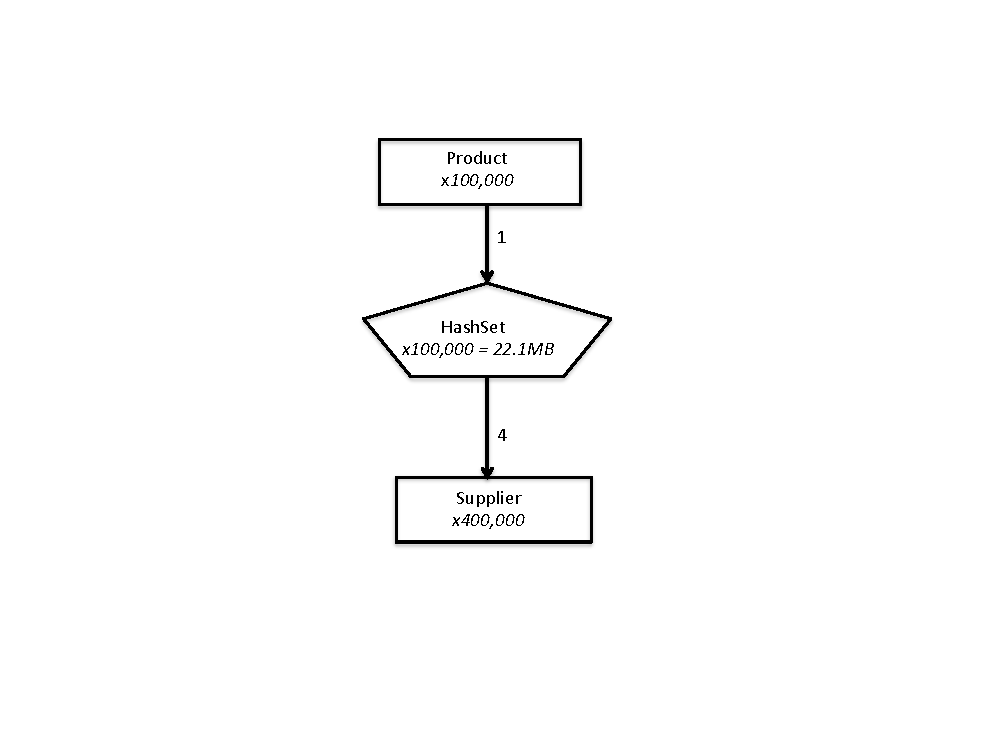
\includegraphics[width=.80\textwidth]{part1/Figures/collections/product-hashset.pdf}
 \caption{A relationship between 100,000 products and alternate suppliers,
  stored as a
  \class{HashSets} of alternate \class{Suppliers} related to \class{Products}.}
  \label{fig:product-hashset}
\end{figure}
%Sun library --  Empty HashSet -- 136 bytes
% 16 bytes HashSet (header + pointer)
% 40 byptes HashMap Object 
% 80 bytes empty array of entries

%HashMapEntry:  24 bytes:  header + 4 fields (value, key, next, hash)
% 4 entries -- 96 bytes
% total overhead for 4 entry hashset: 232 bytes
% 100,000 hashsets with 4 entries is 22.125MB

% HashMap size: 40 for header + 8 for array header
% 24 bytes per entry + 6 per entry in the array (assume extra for growth space)
% so for 100,000 entries, thats 48 + 3,000,000 bytes = 2.86MB
%
% Edge 16*400,000 = 6.4 million = 6.1MB
%
% ArrayList container is 24 bytes (header, size, modcount, pointer) 
% Default array size os 10 -- 10*4+12 = 52 rounds to 56
% ArrayList is 80 (56+24) for 4 entries.
% 400,000 ArrayLists is: 32,000,000 bytes

Using a $HashSet$ for storing the alternate suppliers turns out to be a very
costly decision. The alternate suppliers are represented by 100,000
very small \class{HashSets}, each consuming 232 bytes, which is all overhead.
The total cost is 22.119MB. 
It's hard to think of a good reason why such a heavy-weight collection should ever be used
 for storing just a few entries, and yet, this pattern arises in almost all
 applications. For small sets, \class{ArrayList} is almost always a better choice. 
 \class{HashSet} maintains uniqueness
  and provides fast access, but enforcing uniqueness
is not always needed. If uniqueness is
important, it can be enforced for an \class{ArrayList} 
 with  little extra checking code, and usually without significant performance
 loss when sets are small. Figure~\ref{fig:product-arraylist} shows improved
 memory usage with \class{ArrayList}. Each \class{ArrayList} incurs 80 bytes of overhead,
approximately a third the size of a \class{HashSet}.
 \begin{figure}
  \centering
 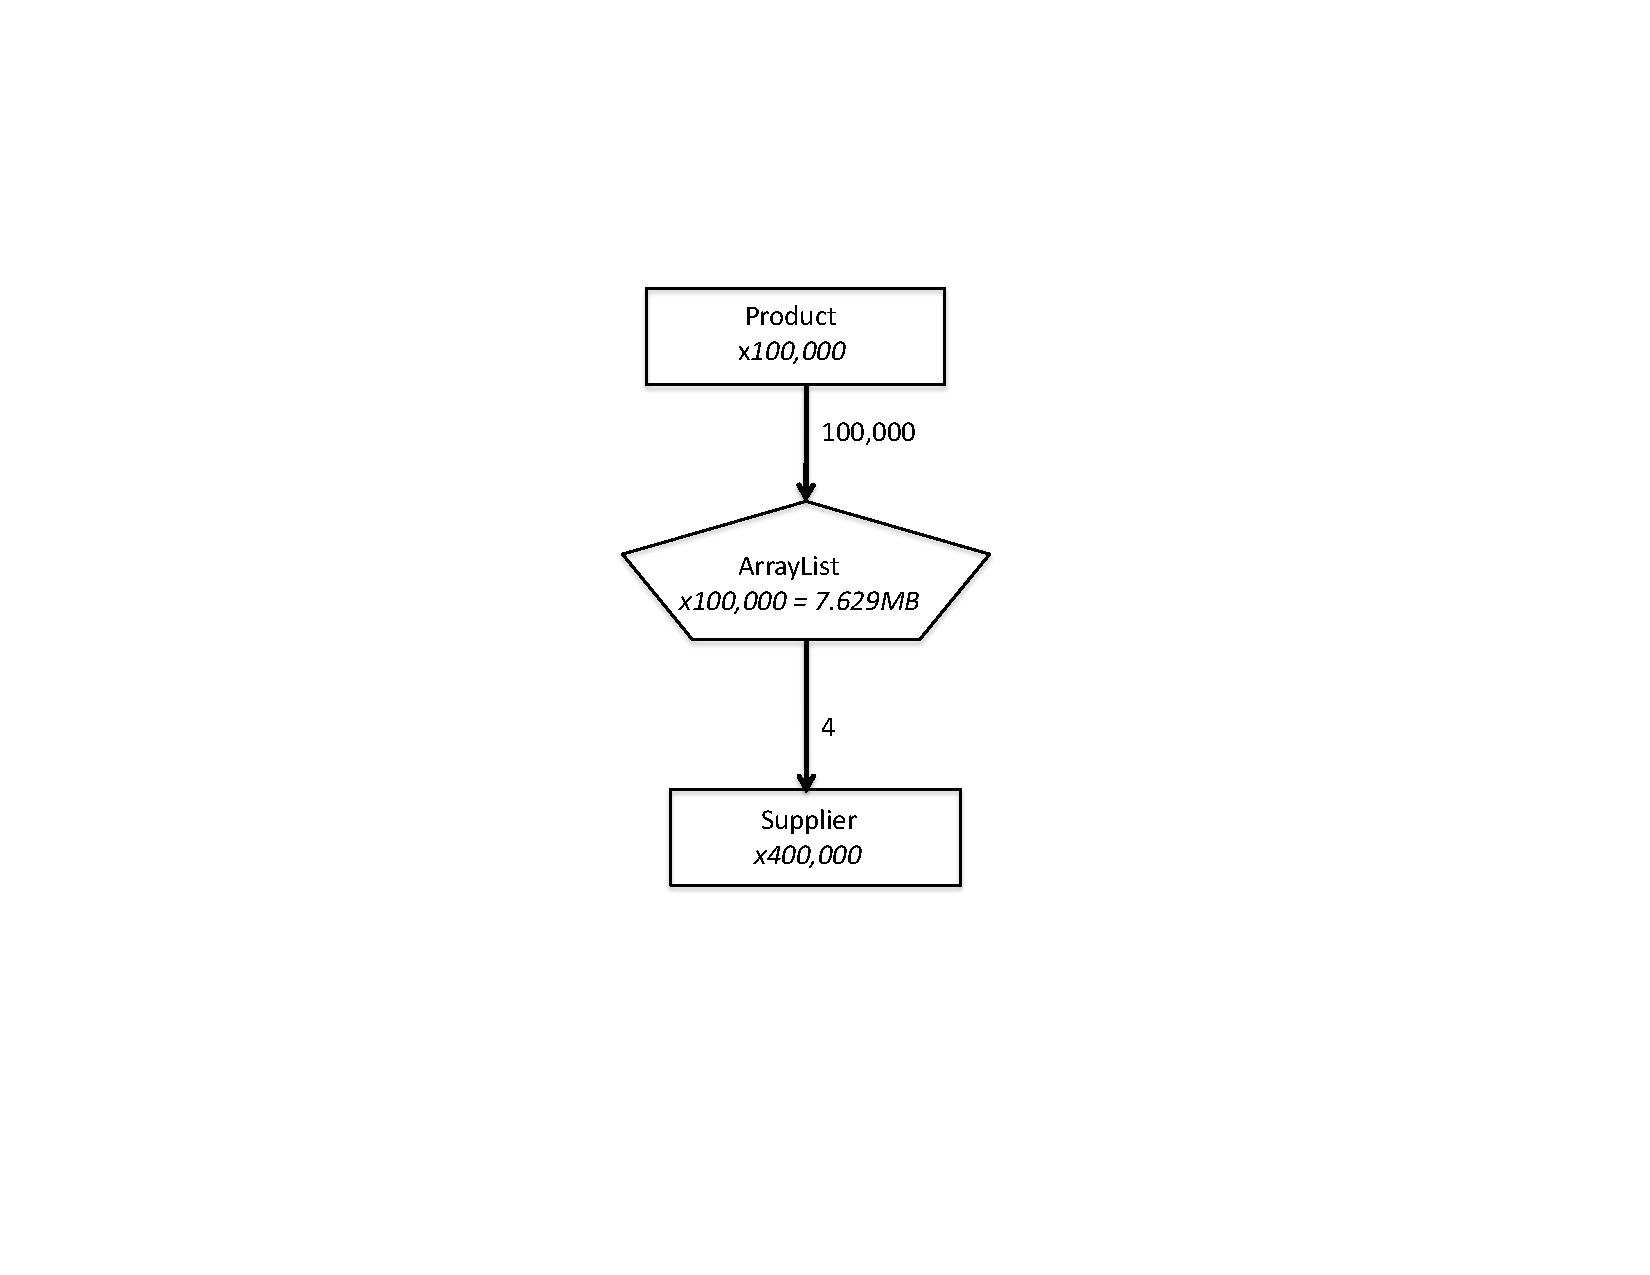
\includegraphics[width=.80\textwidth]{part1/Figures/collections/product-arraylist.pdf}
 \caption{A relationship between 100,000 products and alternate suppliers,
 where the alternate \class{Suppliers} associated with each \class{Product} are
 stored in an \class{ArrayLists}.}
  \label{fig:graph-arraylist}
\end{figure}
This simple change saves 14.49MB. 

Our guess is that the
collection class developers would be surprised by this usage pattern that result
in hundreds of thousands of small $HashSet$. Why bother implementing expandable
structures and clever hashing algorithms for only a few entries?
This mismatch between collection implementation and usage is 
a leading cause of memory bloat. The overhead cost of a $HashSet$ is remarkably
high. Creating many small collections multiplies this basic infrastructure
cost, which is all overhead, filling the heap. 

\section{The Cost Of Collections}
\label{sec:collectioncost}
Let's look at why a \class{HashSet} is so much bigger than an \class{ArrayList}. 
Some of the \class{HashSet} overhead is Java-related and
unavoidable. Other overhead is the result of hard-coded assumptions, for
example, the \class{HashSet} implementation assumes \class{HashSets} will be very large, 
and sacrifices memory space in favor of performance. 
Here is a breakdown of \class{HashSet} design decisions leading to
unnecessary bloat, as illustrated in Figure~\ref{fig:hashset}.
 \begin{figure}
  \centering
 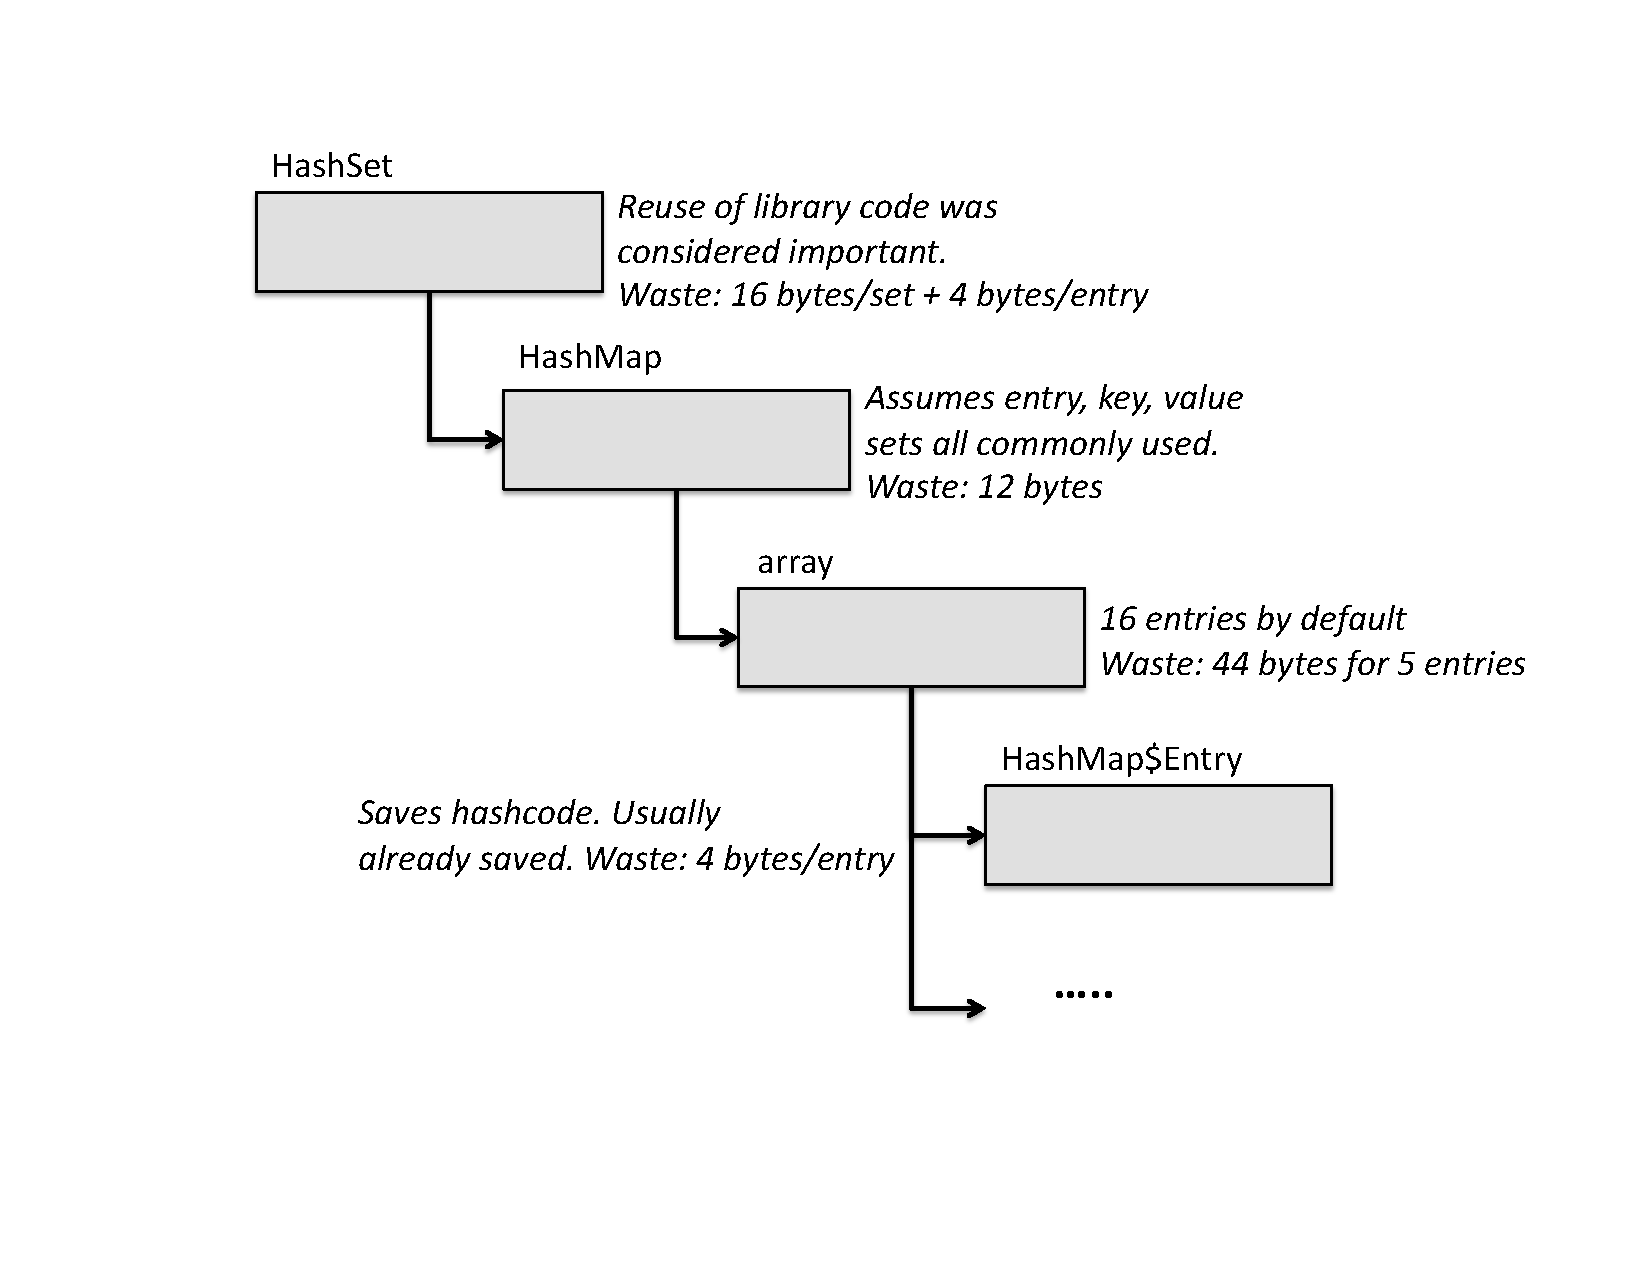
\includegraphics[width=.80\textwidth]{part1/Figures/collections/hashset.pdf}
  \caption{The internal structure of a \class{HashSet} showing how
  implementation assumptions waste memory.}
  \label{fig:hashset}
\end{figure}

\paragraph{Reusing HashMap.} Internally, a \class{HashSet} is just a wrapper,
delegating all of its work to a \class{HashMap}.
This decision to reuse the \class{HashMap} code instead of specializing
\class{HashSet} costs an extra 16 bytes, which is reasonable if
\class{HashSets} are big and the fixed overhead costs are amortized away. 
Unfortunately, the fixed cost is multiplied when there are many
small \class{HashSets}. 
Also, \class{HashMap} is more general than what is needed for a \class{HashSet}.
Each \class{HashMap\$Entry} stores a key and a
value, and \class{HashSet} only uses the key, so four bytes are wasted per
entry. Sometimes specialization is a better option than reuse, especially for
library classes, where the usage patterns are not known in advance.
  
\paragraph{Open Chaining.} \class{HashMap} itself is fairly
 expensive. First, the \class{HashMap} object is just a container pointing
 to the actual array of entries. This delegation is necessary in Java.
 Secondly, \class{HashMap} uses an
 open chaining algorithm, which means that clashing entries are chained in a
 linked list. With open chaining, each entry requires its own
 \class{HashMap\$Entry} object and an extra level of indirection.
 
\paragraph{Default Array Size.} 
A \class{HashMap}, which is used to implement a \class{HashSet}, has a default
size of 16 entries, which means that its array of entries has an initial
size of 16. This wastes space when most \class{HashSets} have only a few
entries. For example, a \class{HashSet} with five entries wastes 44 bytes.


\paragraph{Bookkeeping Fields.} \class{HashMap} allows callers to iterate over
its set of keys, set of values, and set of entries. These sets are cached once
they are created. Every \class{HashMap} has three pointers
to store these sets, which is an extra 12 bytes.
However, its not that common to use
any of these sets, and very rare to use more than one set at a time.
 Certainly when the \class{HashMap} is part of a \class{HashSet}, 
there is never a need for a set of values.
  
 \paragraph{Extra Per-Entry Costs.} Each \class{HashMap\$Entry} stores a
 hashcode, which is an unnecessary redundant field. The most common keys are either
 \class{Strings}, which store their own hashcode, or \class{Integers}, whose
 hashcodes are easy to compute. 
\paragraph{}
In contrast, \class{ArrayList} has a smaller fixed cost and a smaller
per-entry cost than \class{HashSet}. It is really just an expandable array,
consisting of a wrapper object and an array of entries, as shown in Figure~\ref{fig:arraylist}. 
Lower fixed cost means that an \class{ArrayList} with just a few
 elements is smaller than a \class{HashSet} with the same elements. Fixed costs
 include wrapper objects and unitialized array elements. The fact that \class{HashSet}
 delegates to \class{HashMap} dramatically inflates its fixed cost. 
 \begin{figure}
  \centering
 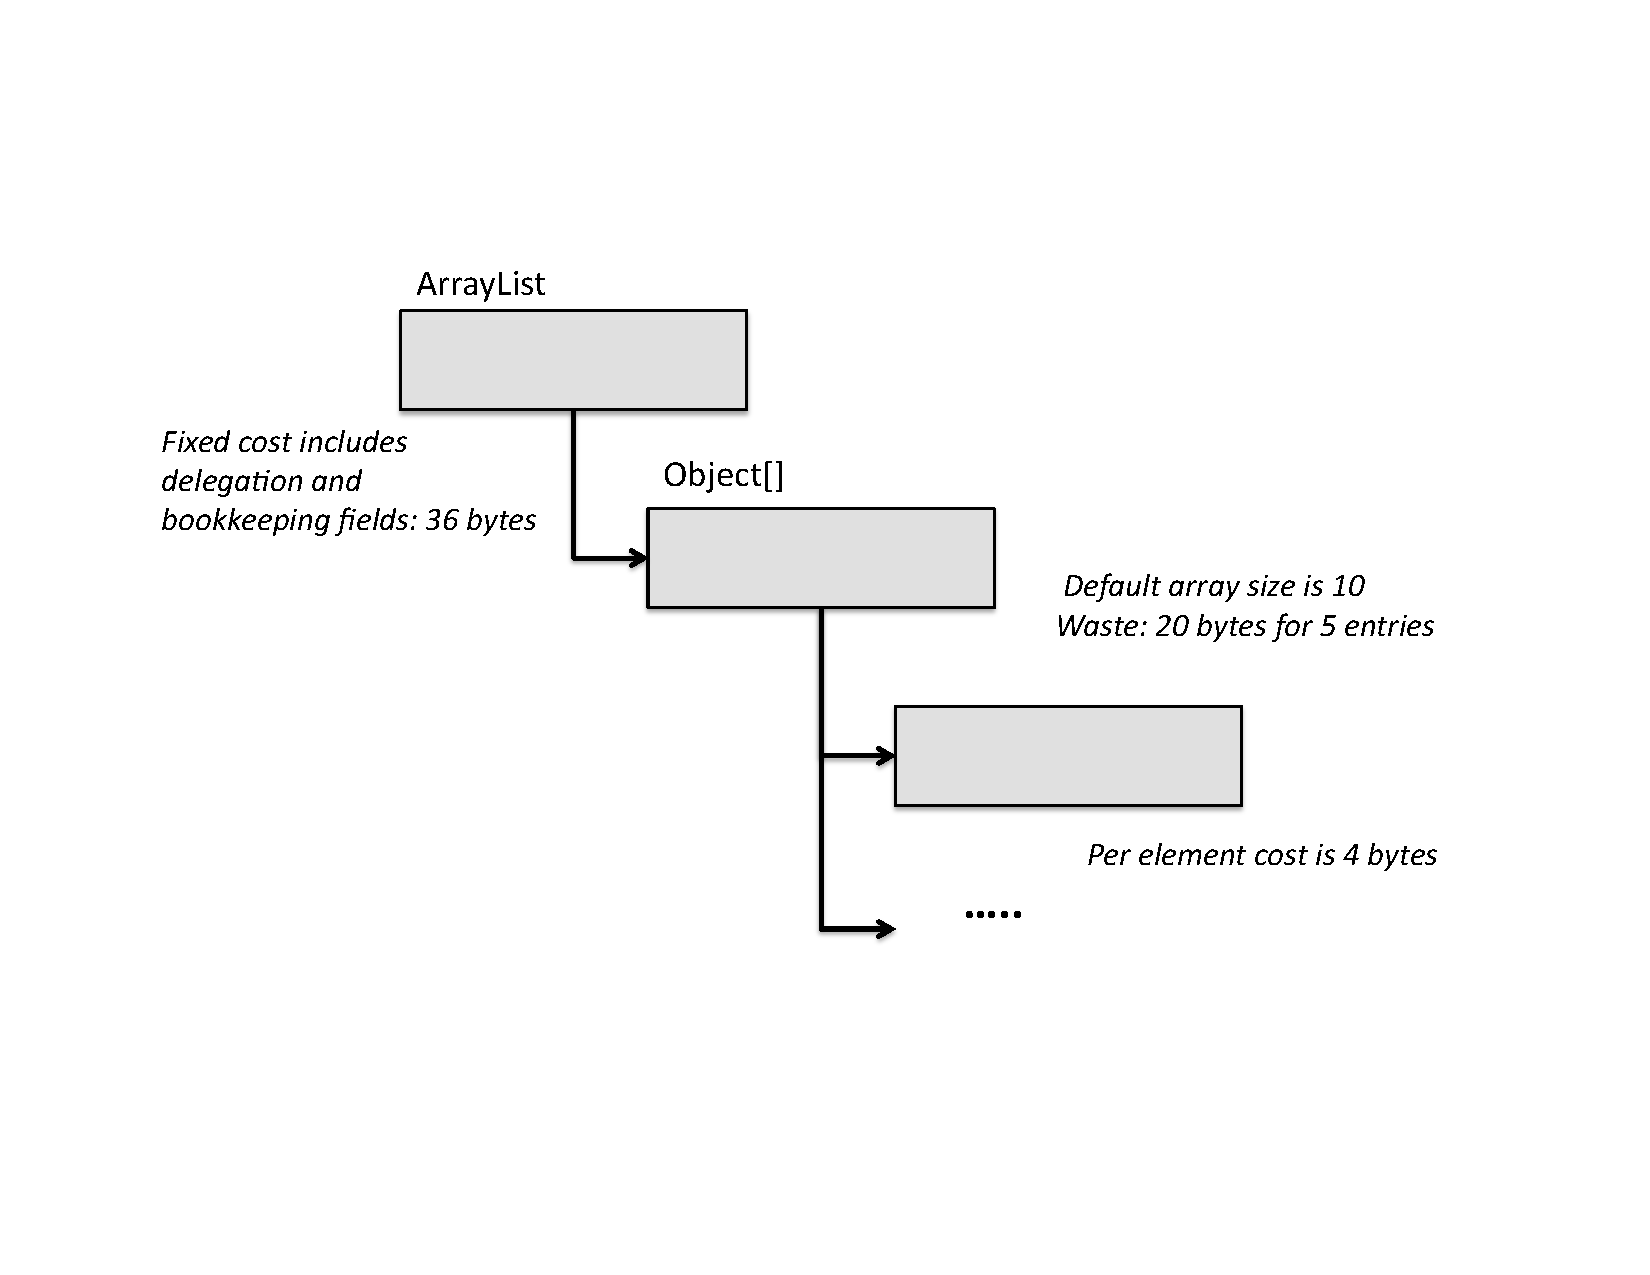
\includegraphics[width=.80\textwidth]{part1/Figures/collections/arraylist.pdf}
  \caption{The internal structure of an \class{ArrayList}, which has a
  relatively low fixed overhead, and is scalable.}
  \label{fig:arraylist}
\end{figure}
 Lower per-entry cost means that
 \class{ArrayList} scales much better than \class{HashSet}. The per-entry cost
 of an \class{ArrayList} entry is an entry array pointer, which is 4 bytes.
 The per-entry cost of a \class{HashSet} is an entry array pointer plus a
 \class{HashMap\$Entry}, which is 28 bytes. So \class{ArrayList}  is better
 both for small and large sets.

Table~\ref{tab:collection-costs} shows the empty-collection costs of four basic
collections, \class{ArrayList}, \class{LinkedList}, \class{HashMap}, and \class{HashSet}. These costs have been
calculated based on the Sun JVM, using the techniques
described in Chapter~\ref{chapter:delegation}. The various other Java standard
library implementations in circulation have costs
similar to these. You can calculate them using the same methodology.

\begin{table}
  \centering
 %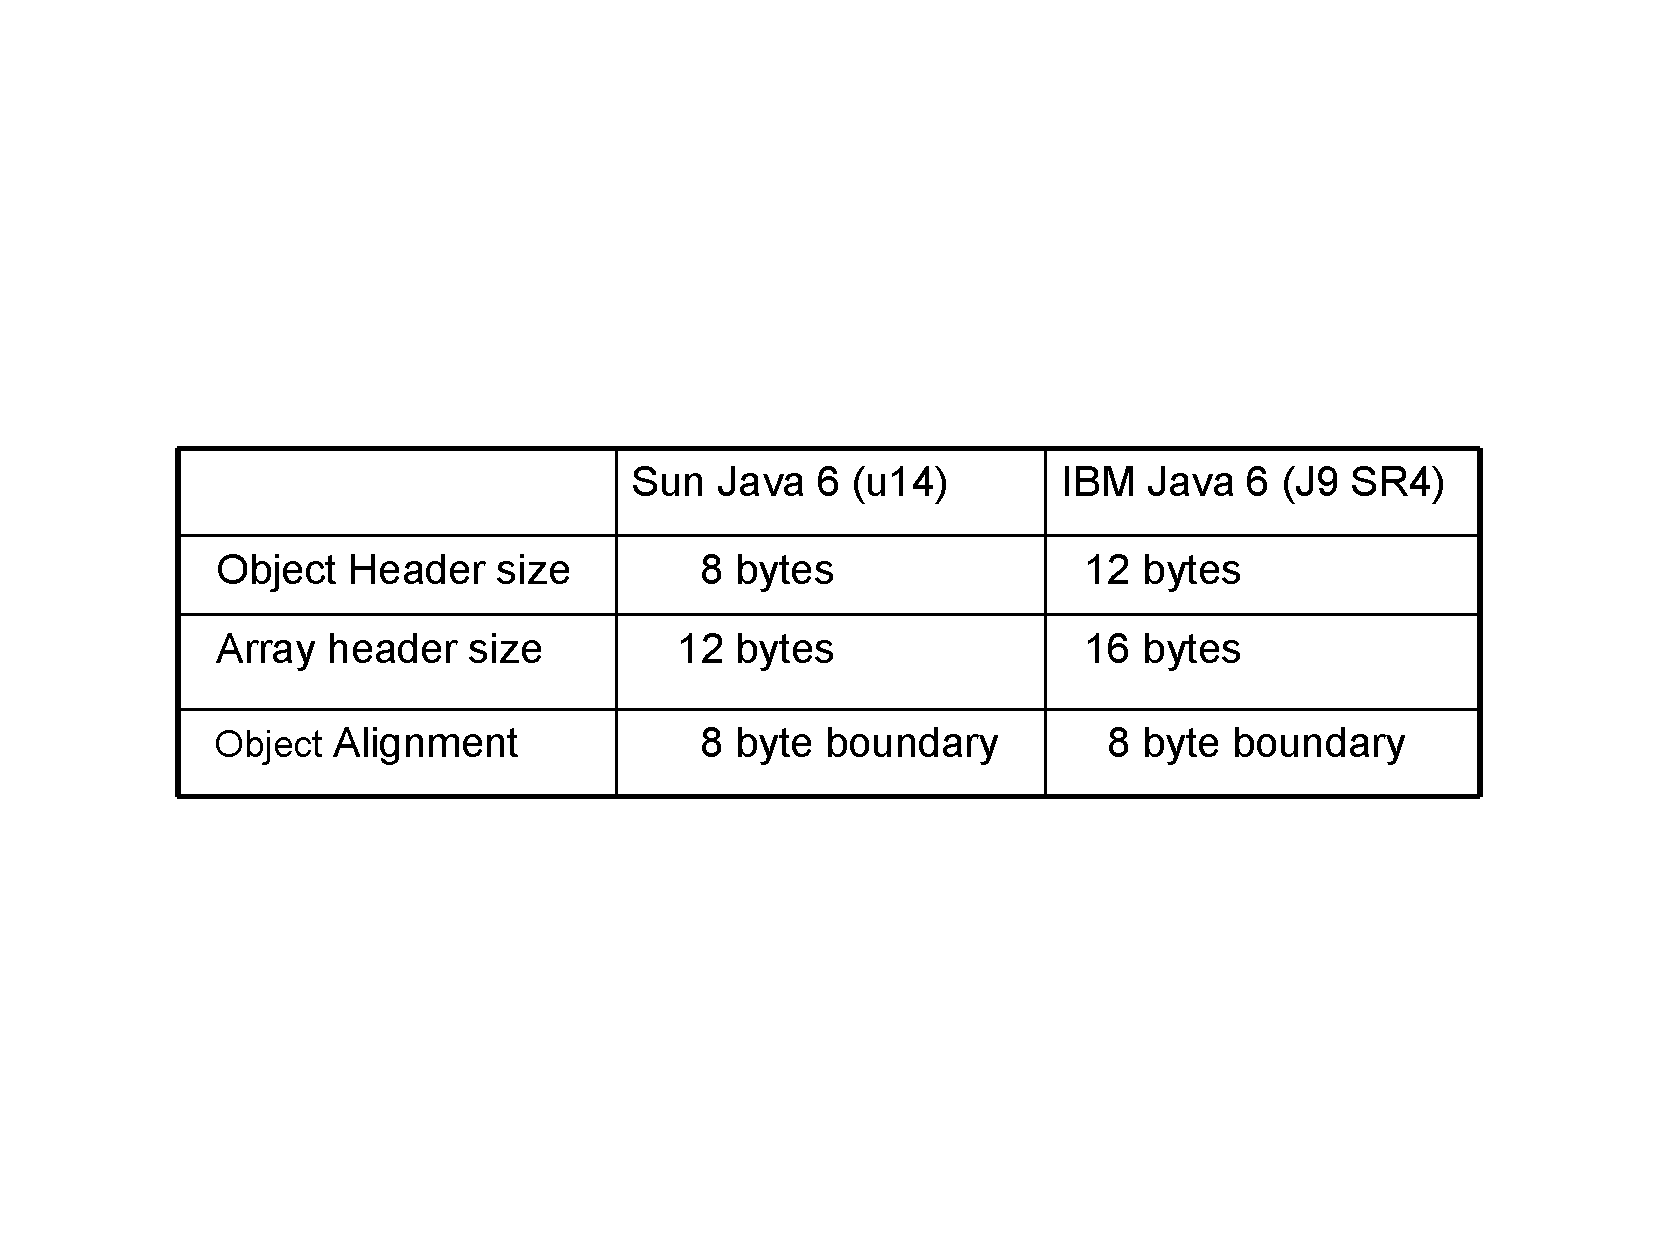
\includegraphics[width=.70\textwidth]{part1/Figures/modelingdatatypes/object-overhead.pdf}
 % 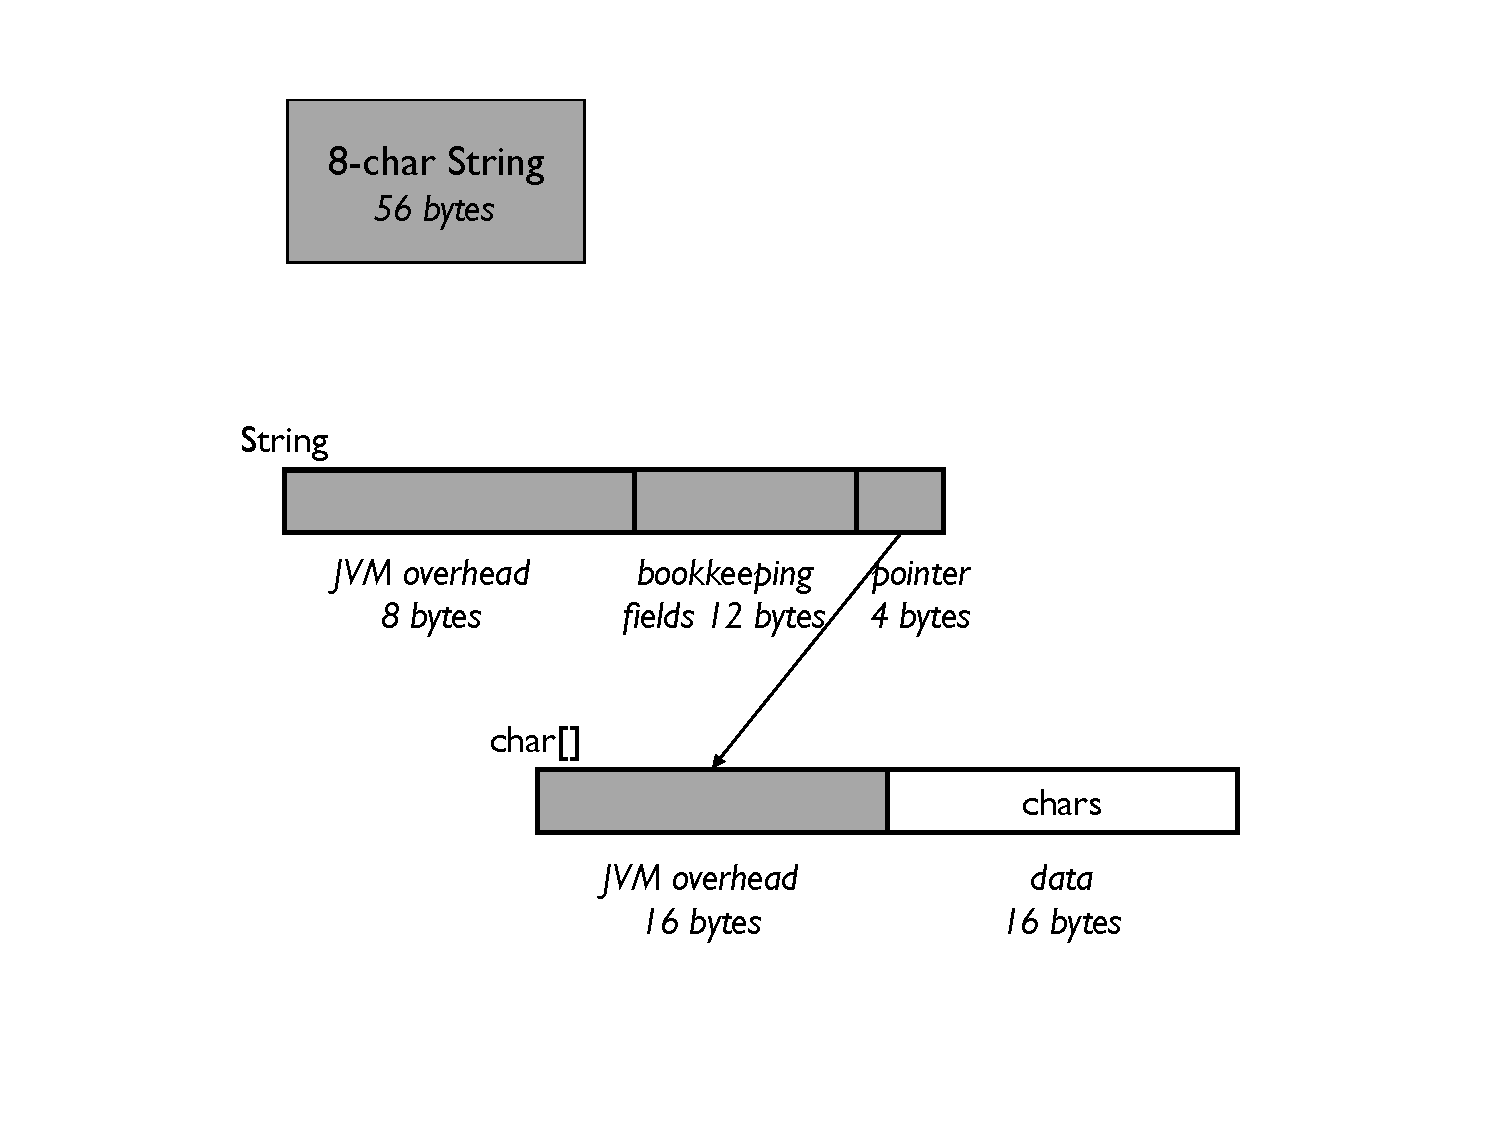
\includegraphics{eight-char-string}
 \begin{tabular}{llll} \toprule
 	 Collection & Fixed Cost & Per-Entry Cost & Default Capacity \\ \midrule
 	ArrayList & 80 bytes & 4 bytes & 10 entries \\
 	LinkedList & 48 bytes & 24 bytes & 1 sentinel entry \\
 	HashMap & 120 bytes & 28 bytes & 16 entries \\
 	HashSet & 136 bytes & 28 bytes & 16 entries \\
 	\bottomrule
 \end{tabular}
  \caption{The cost breakdown of four basic Java standard library collections
  with default size and no entries. The fixed cost includes an array whose
   size equals the default capacity. The per-entry cost is used to
  determine scalability.}
  \label{tab:collection-costs}
\end{table} 

\section{Properly Sizing Collections}
\label{sec:proper-size}

Collections such as \class{HashMap} and \class{ArrayList} store their entries in
arrays. When these arrays become full, a larger array is allocated
and the entries are copied into the new array.  Since allocation and copying
can be expensive, these entry arrays are always allocated with some extra
capacity, to avoid paying these growth costs too often. 
This is why the initial capacity of an \class{ArrayList} is 10 rather than zero
 or one, and why its capacity increases by
50\% when it is reallocated. 
Similarly, the capacity of a \class{HashMap} starts at 16, and grows by a
factor of 2 when the \class{HashMap} becomes 75\% full. 

These default policies trade space
for time, on the assumption that collections grow. However,
typical applications have hundreds of thousands of small collections that
don't grow. As a result, there is no performance gain, and the extra
empty array slots can add up to significant bloat problem. Unless you take explicit
action, element arrays are almost always too big.

 
 Fortunately, for \class{ArrayLists}, it is possible to right-size them. If you
 know that an \class{ArrayList} has a maximum size $x$ less than the default
 size, then it's worth passing $x$ as a parameter to the constructor. This sets the initial capacity of the
 \class{ArrayList} to $x$. However, if you are wrong and the \class{ArrayList}
 grows bigger than $x$, then it will grow by 50\%, which may
 be worse than just taking the default initial size.
 
 Alternatively, you can call the \code{trimToSize} method which shrinks the
 entry array by eliminating the extra growth space. Trimming reallocates and
 copies the array, so it is expensive to keep calling \code{trimToSize} while an
 \class{ArrayList} is still growing. Trimming is appropriate after
 it has been fully constructed and will never grow again. In fact, applications
 often have a build phase followed by a used phase. 
 \class{ArrayLists} can be trimmed
  between these two phases, so that the cost of reallocation and copying is
  paid only once.
 
 Returning to the graph example, all
 \class{ArrayLists} in Figure~\ref{fig:graph-arraylist} have the default
 capacity. If we assume that the the graph is built in one phase, and used in
 another phase, then it is possible to trim all of the \class{ArrayLists}.
 This should save quite a bit of space, since there are 100,000
 \class{ArrayLists} with four entries on average, and 400,000
 \class{ArrayLists} with two entries each. In fact, trimming these
 \class{ArrayLists} saves 15.2 million bytes, as shown in
 Figure~\ref{fig:trimmed-graph}. The total size is reduced by 25.6\%.
 % 100,000 4 entry arrays == a 4 entry array is 32 bytes (16+12=28, rounds up
 % to 32)
 % So each array saves (56-32)=24 bytes.  100,000*24=2,400,000 bytes saved
 % = 1,600,000 bytes
 % 400,000 * (10-2)*4 = 12,800,000 byptes/ saves 32 bytes per arraylist
 % 32*400000=12,800,000 saved   32,000,000 - 12,800,000 = 19,200,000

 \begin{figure}
  \centering
 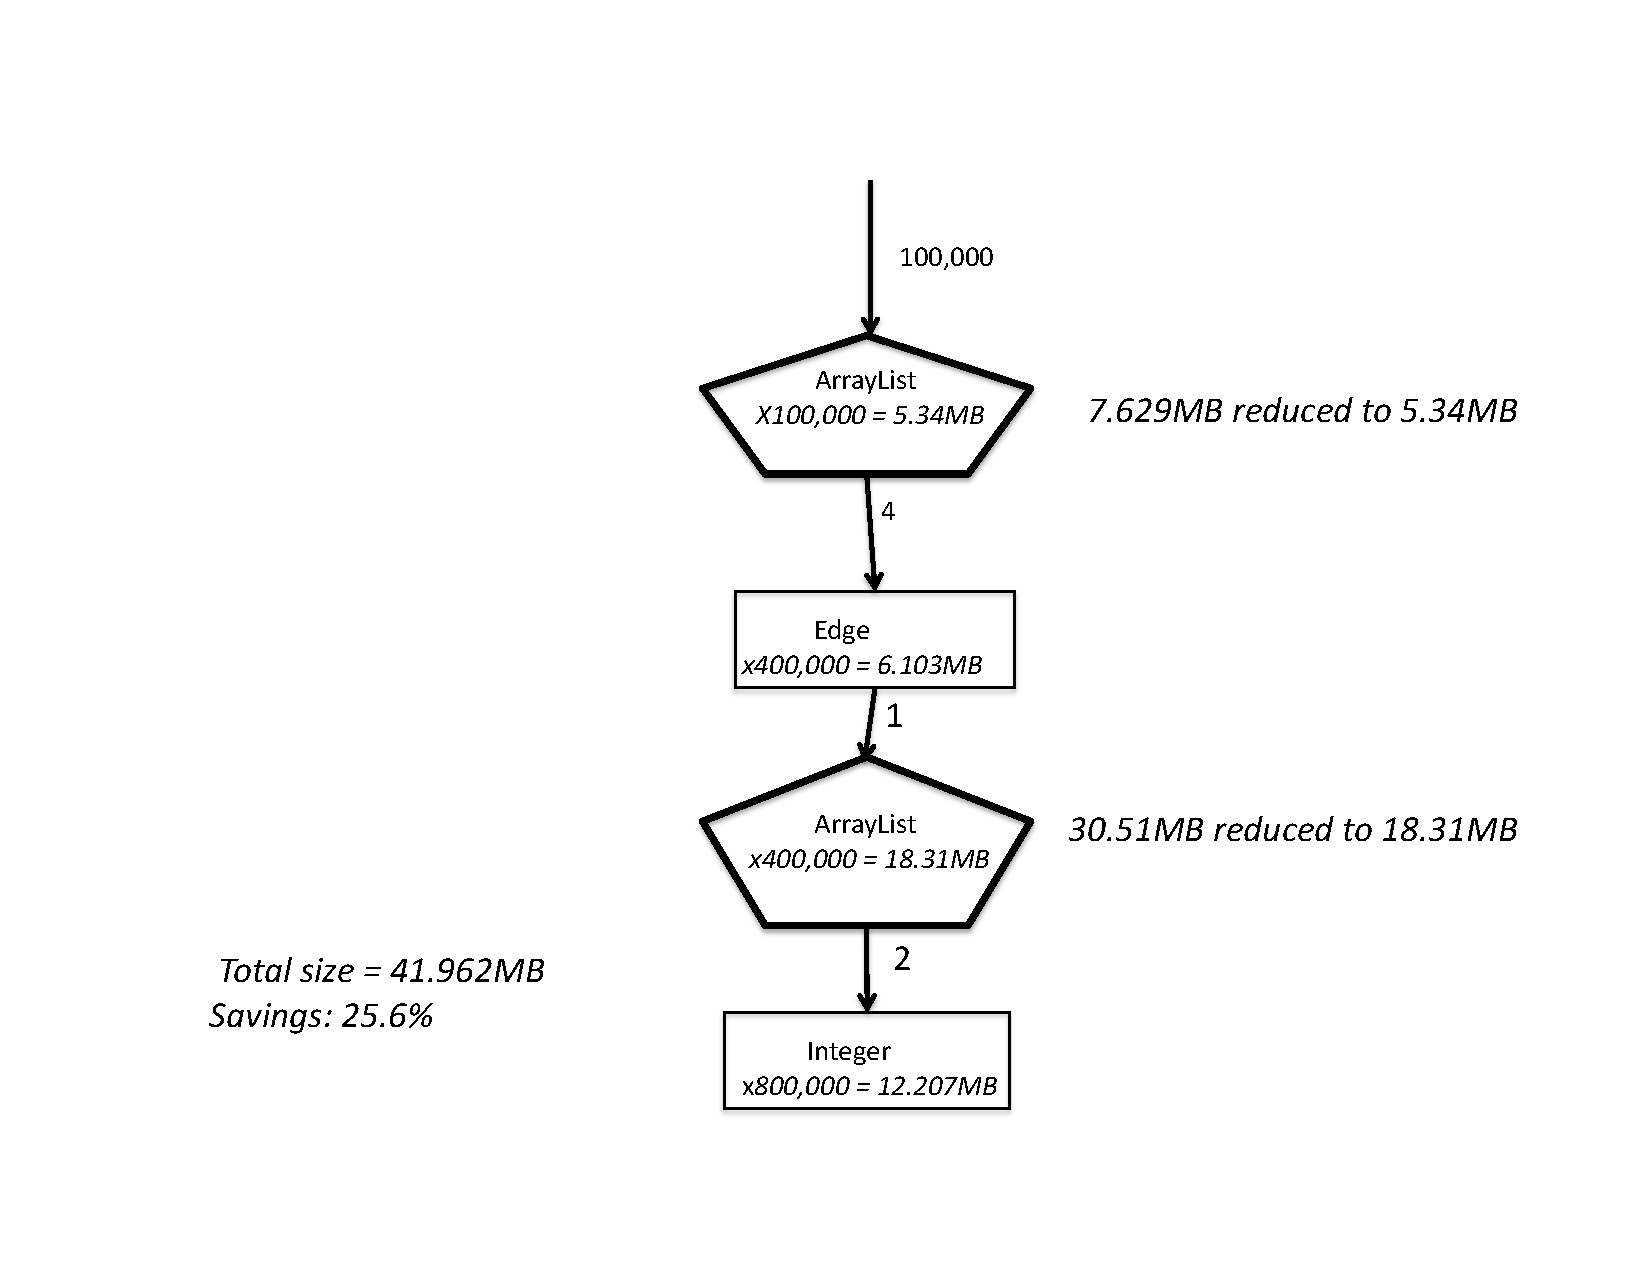
\includegraphics[width=.80\textwidth]{part1/Figures/collections/trimmed-graph.pdf}
  \caption{The graph example after all of the \class{ArrayLists} have been
  trimmed by calling the \code{trimToSize} method.}
  \label{fig:trimmed-graph}
\end{figure}
 
\class{HashSets} and \class{HashMaps} do not have \code{trimToSize} methods,
but it is possible to pass the initial capacity and load factor as constructor
parameters when creating a \class{HashSet} or \class{HashMap}. 
However, before changing the initial capacity, you should
ask yourself whether using a \class{HashSet} or \class{HashMap} is a
wise decision in the first place. If you are going to end up with many
collections with fewer than 16 elements, perhaps there is a more memory-efficient solution, like
\class{ArrayList}.
  
A \class{LinkedList} is another alternative for small collections, and are
better than \class{ArrayLists} if the collections are changing a lot. The
24 byte per-entry cost is larger, but there is no element array, and only one
extra entry, which is a sentinal.

\section{Avoiding Empty Collections}

Too many empty collections is another common problem that fills up space in the
heap. A quick look inside an empty collection shows that it is not all that
empty. According to Table~\ref{tab:collection-costs}, an empty \class{HashMap} consumes
120 bytes, and an empty \class{ArrayList} consumes 80
bytes, assuming a default initial size. 
Even if the initial size is zero, empty collections are still
large. A zero-sized \class{HashMap} consumes 56 bytes, and a zero-sized
\class{ArrayList} consumes 40 bytes. Empty \class{HashSets} are even bigger.

Empty collection problems are generally caused by eager initialization, that is,
allocating collections before they are actually needed. Exacerbating this
problem, collections themselves also allocate their internal objects in an eager
fashion. For example, \class{HashMap} allocates its entry array before any entries are inserted.
You might think that eager initialization is not such a big problem, since
entries will be added eventually. However, often collections are allocated
just in case they are needed later, and remain empty throughout the execution.

Suppose the graph
in Figure~\ref{fig:trimmed-graph} is initialized by the code:
\begin{shortlisting}
ArrayList nodes;
HashMap graph;
int numNodes;
   ..
   public void initGraph() {
       ..
       for (i = 0; i < numNodes; i++) {
          graph.put(nodes.get(i), new ArrayList());
       }
   }
\end{shortlisting}
Initially, each node is mapped to an empty edge \class{ArrayList}, so there
are 100,000 empty \class{ArrayLists} before any edges are inserted.
As the graph is populated, many of these \class{ArrayLists} will become
non-empty, but it is likely that a good number of nodes have no edges. 
If 25\% of the nodes in the final graph still have no edges, there will be
25,000 empty \class{ArrayLists}, which consume .95MB after calling
\code{trimToSize}. Figure~\ref{fig:empty-array} shows the entity-collection
diagram after removing 25,000 empty edge \class{ArrayLists}. Note that
there are now only 75,000 edge \class{ArrayLists} shown, and since there are
no more empty \class{ArrayLists}, the average fanout increases to 5.33. 
\begin{figure}
  \centering
 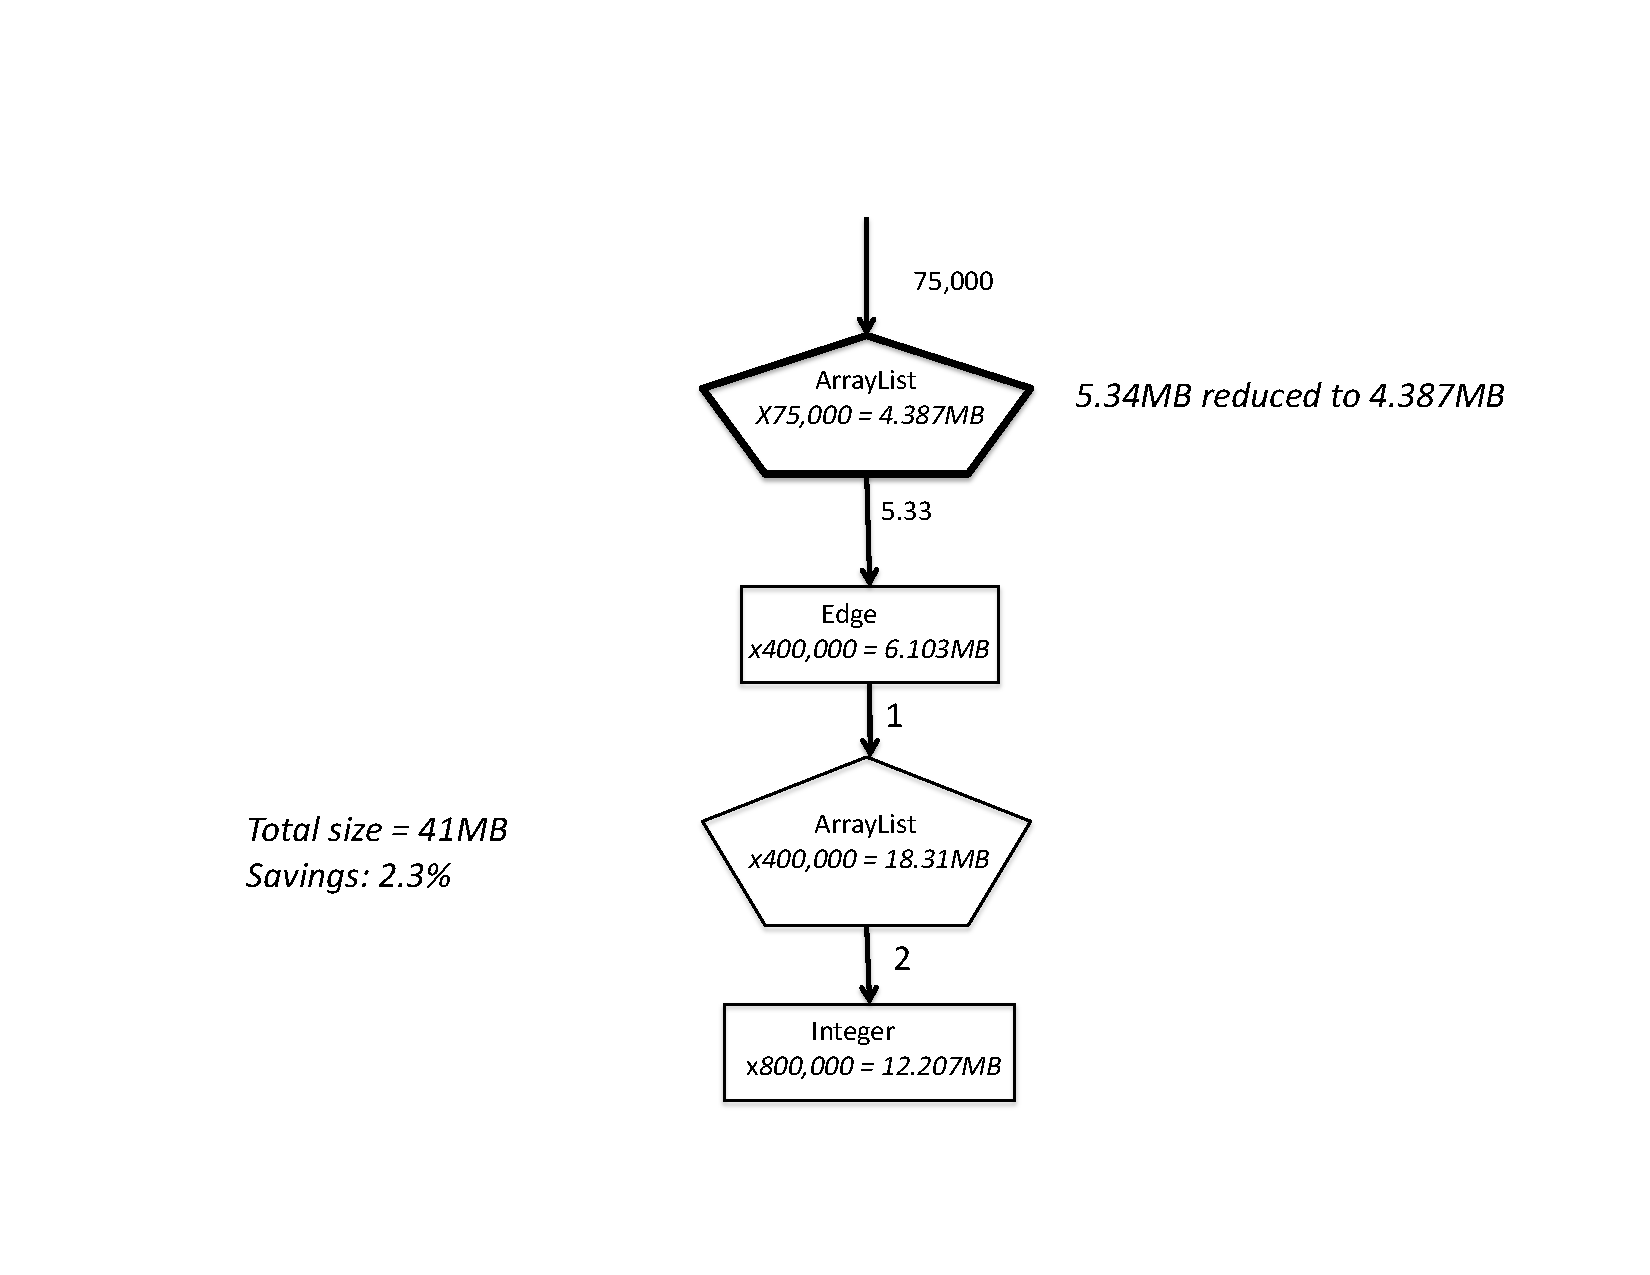
\includegraphics[width=.80\textwidth]{part1/Figures/collections/empty-array.pdf}
  \caption{The graph example without empty \class{ArrayLists}.}
  \label{fig:empty-array}
\end{figure}
 
 Delaying allocation prevents creating too many empty collections.
 That is, instead of initializing all of the collections that you think you
 may need, allocate them on-demand, just before inserting an edge. On-demand
 allocation requires more checking code, to avoid \code{NullPointerExceptions}.
 
 Alternatively, you can initialize collection fields to reference static empty collections,
 including EMPTY\_SET,
 EMPTY\_LIST, and EMPTY\_MAP. For example, 
 calling static method \code{Colletions.emptyList} to initialize edge
 \class{ArrayLists} maps all nodes to a singleton immutable static
 \class{ArrayList}, so that no empty \class{ArrayLists} are created:
 \begin{shortlisting}
 public void initGraph() {
       ..
       for (i = 0; i < numNodes; i++) {
          graph.put(nodes.get(i), Collections.emptyList());
       }
   }
 \end{shortlisting}
This initialization avoids the need to check whether an \class{ArrayList}
exists at every use. For example, the size method and iterators will just work.
However, you have to be careful not to let any references to static empty
collections escape its immediate context. 
If you give out a reference to a static empty collection, 
then there�s no way to update this escaped empty-collection reference
once an actual collection is allocated. 

\section{Fixed Size Collections}

Java collections can grow to be
arbitrarily big, but this functionality comes at a cost.
Collections include wrapper objects, and 
may be sized with extra growth room. If
you know that the size of a collection is fixed, having the ability to expand
the collection is unnecessary, and it is better to choose a cheaper alternative.
In fact, often you can use a
simple Java array, and not use a collection at all.  

Let's look more closely at an \class{Edge} in the graph example in
Figure~\ref{fig:edges}(a). An \class{Edge} object is a wrapper containing an
 \class{ArrayList}, which is just another
wrapper pointing to an \class{Integer} array. 
Since an \class{Edge} will never hold more than two \class{Integers}, it isn't 
necessary to store these in an \class{Arraylist} --- a simple array will do.
This change, eliminating the \class{ArrayList} object, removes 24 bytes per
\class{Edge}, as shown in Figure~\ref{fig:edges}(b), adding up to 9.16MB.
\begin{figure}
  \centering
 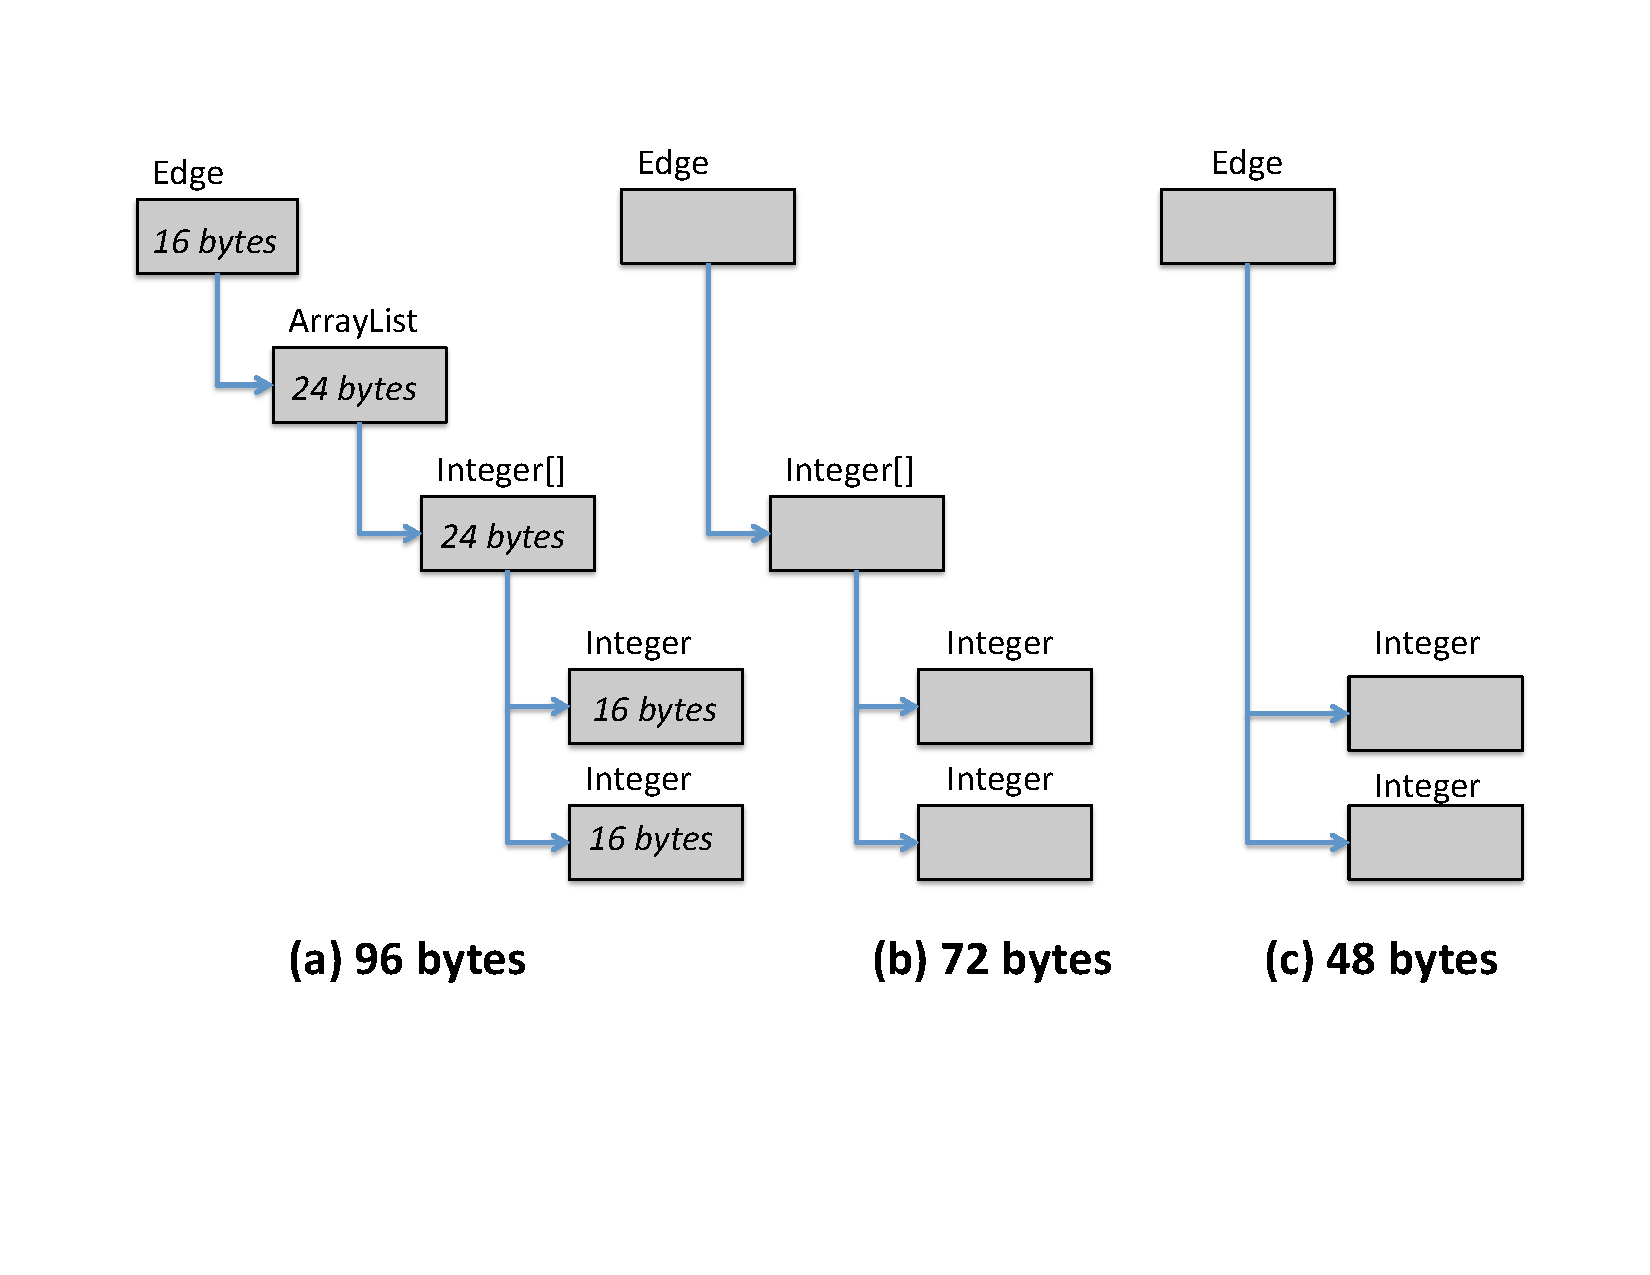
\includegraphics[width=.80\textwidth]{part1/Figures/collections/Edges.pdf}
  \caption{(a) An \class{Edge} has 96 bytes. (b) Replacing the
  \class{ArrayList} by an array eliminates 24 bytes. (c) Inlining the array
  eliminates another 24 bytes.}
  \label{fig:edges}
\end{figure}
This is an example of choosing an overly-general collection. In
this situation, you don't need a collection at all. Using \class{ArrayList}
for storing fixed- or bounded-size arrays is a
common practice that can be easily avoided.

There is one final optimization that can be performed on the \class{Edge}
class. Namely, making the two \class{Integers} fields of \class{Edge} instead
of elements of an array, as shown in Figure
Figure~\ref{fig:edges}(c). This optimization eliminates the
array object, which saves another 24 bytes per edge, which is another 9.16MB.


In effect, these two steps have
transformed a dynamic representation of a type, where field values are stored in
arrays or \class{ArrayLists}, into a static representation, namely, a class.
Using fixed-size arrays or \class{ArrayLists} to store fields is a typical
pattern in Java. For example, when reading records from a database, it is a
common practice to store the data fields of a record in an array or
\class{ArrayList}. If you do not know that the fields are until execution, then
this representation makes sense. 
Even though this representation introduces extra objects, there is often no alternative.
However, if you do know the structure in advance, it is far better space-wise
to inline these fields in a class definition,

The resultin g entity-collection diagram for the graph example is shown in
Figure~\ref{fig:arraylist-to-array}. The total size, from the first
entity-collection diagram in Figure~\ref{fig:graph-hashset}, has been reduced
by 68\% , which is quite significant. The bloat factor has gone from 95.7\% to
86.6\%. You might wonder why the bloat factor is still so high? The answer
is that the overhead of nesting an \class{ArrayList} in a \class{HashMap} is
still very high compared to the data, which is just two \class{Integers}. There
is still one more simple optimization that can be performed, namely, replacing
the \class{Integers} by primitive \code{int} fields in \class{Edge}.
Calculating the bloat factor after making this transformation is left as an
exercise for the reader.
\begin{figure}
  \centering
 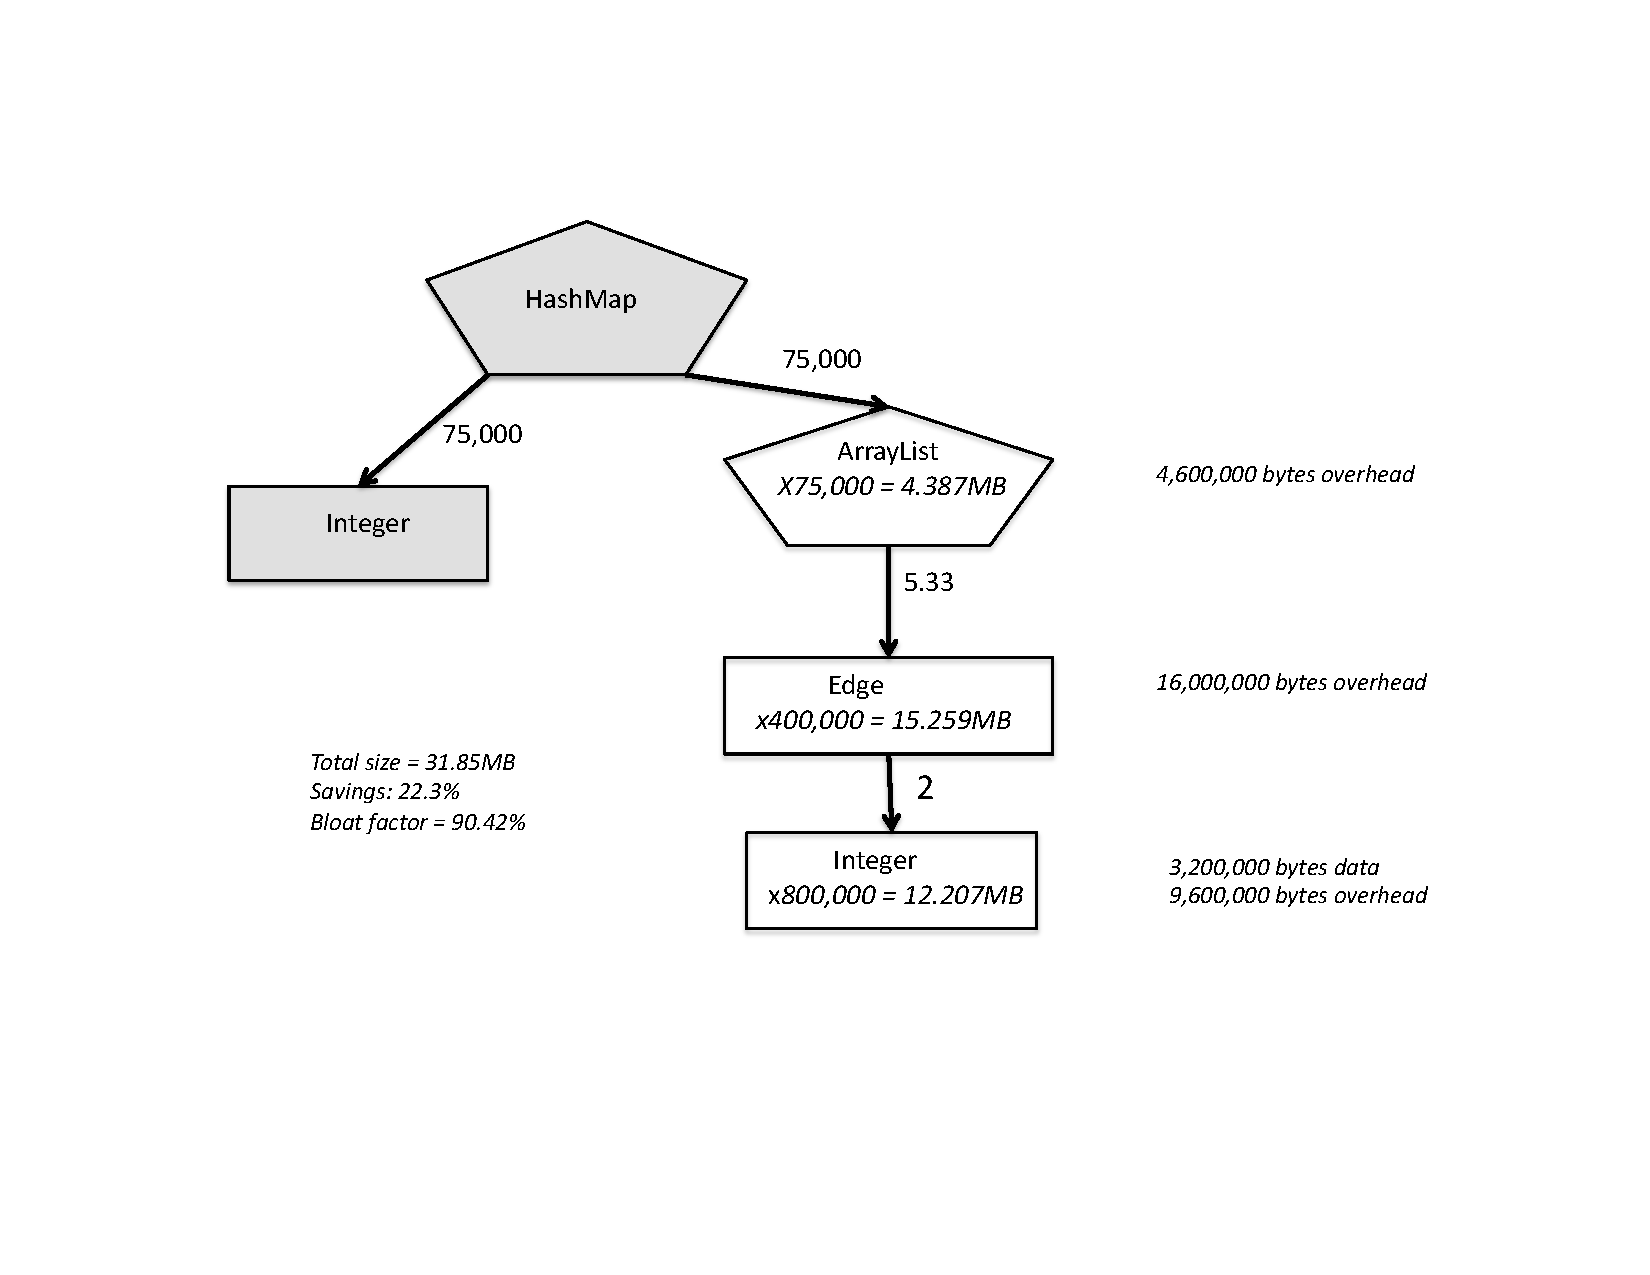
\includegraphics[width=.80\textwidth]{part1/Figures/collections/arraylist-to-array.pdf}
  \caption{Final entity-collection diagram for the graph example.}
  \label{fig:arraylist-to-array}
\end{figure}

\section{Summary}

This chapter describes a number of ways to mitigate high memory costs when your
program has many small collections:
\begin{itemize}
  \item Choose the most memory-efficient collection for the job at hand. In
  particular when collections have at most a few elements in them, you don't
  need expensive functionality like hashing. 
  \item Make sure collections are properly sized. If you know that a collection
  will not grow any more, then there is no reason to maintain extra room for
  growth.
  \item Avoid lots of empty collections. It is common to allocate collections 
 ahead of time, whether or not they will eventually ever be used. If you
 postpone creating them until they are needed, often you will end up with fewer collections, 
 and no empty collections.
 \item Use arrays instead of \class{ArrayLists} when you know the maximum size
 of the \class{ArrayLists} in advance.
 \item Avoid dynamic types, where field values are stored in arrays or
 \class{ArrayLists} instead of object fields, if possible. It's better to use a
 class to represent a type, if the type is really static.
\end{itemize}

Small collections have a fixed-size overhead, which is there as soon as the
collection is allocated. Fixed costs are amortized when collections are big,
but when they have only a few elements, the fixed overhead dominates the memory
cost. The fixed costs of collections is provided in
Section~\ref{sec:collectioncost} to help you make an informed choice. 
Next chapter looks at per-entry costs of larger collections and nested
collections.
 



